\subsection{Orbit length \label{sec:ringlen}}

Recombination process relies on to the $10^{-5}$ level control of 
beam time of flight in the CR. 
The 3~GHz RF phase monitor (BPR) provided its direct measurement when a short pulse
(shorter then the ring circumference) was stored in the ring for many turns.
The phase of the reference signal was adjusted such that signal was zero for the first turn.
%Figure~XX shows how its signal is expected to be in case of perfect ring length and 5\% error.
%The spectrim of the 
If the ring length was correct, the signal 
\begin{itemize}
 \item  had maximum amplitude for the 2nd turn,
 \item  was zero for the 3rd turn,
 \item  had minimum amplitude for the 4th turn,
\end{itemize}
This pattern was repeated for for the remaining turns.
The powering of the wiggler was than adjusted to find a good setting.
% or the main bending magnets or all quadrupoles 

Much more accurate measurement was achieved by performing FFT of the BPR signal.
When the ring length is correct for recombination factor 4, 
the spectrum contains the first peak at $\frac{1}{4} f_{rev}$, 
where $f_{rev}$ is the revolution frequency, and
secondary peaks are spaced by $\frac{1}{2} f_{rev}$.
If the ring length is longer, the odd peaks shift towards 
lower frequencies and the even ones towards higher frequencies.
When the length becomes multiple of $\lambda_{RF}$ the first peak disappears
and 2nd and 3rd peak merge at $f_{rev}$.
Average of 2nd and 3rd peak gives the revolution frequency.
Frequency difference between these peaks, $\Delta f$, is directly proportional
to the ring length modulo the RF wavelength: 
$L_{frac} = \frac{\lambda_{RF}}{4} \cdot (1 - \frac{ 2 \Delta f}{f_{rev}})$

Example of the measured spectra is presented in Figure~\ref{fig:crlenbprspectrum}. 
Figure~\ref{fig:crlen} shows measured fractional ring length $L_{frac}$ 
in function of the wiggler powering. The dependence was exactly as it was predicted. 
In this particular measurement the ring length was 1.5~mm different from the nominal value. 
The value of the offset naturally depended on how well the closed orbit is corrected
and it was always well within the limits of the required operational range.

\begin{figure}[!h]
\centering
\subfloat[]
 {
  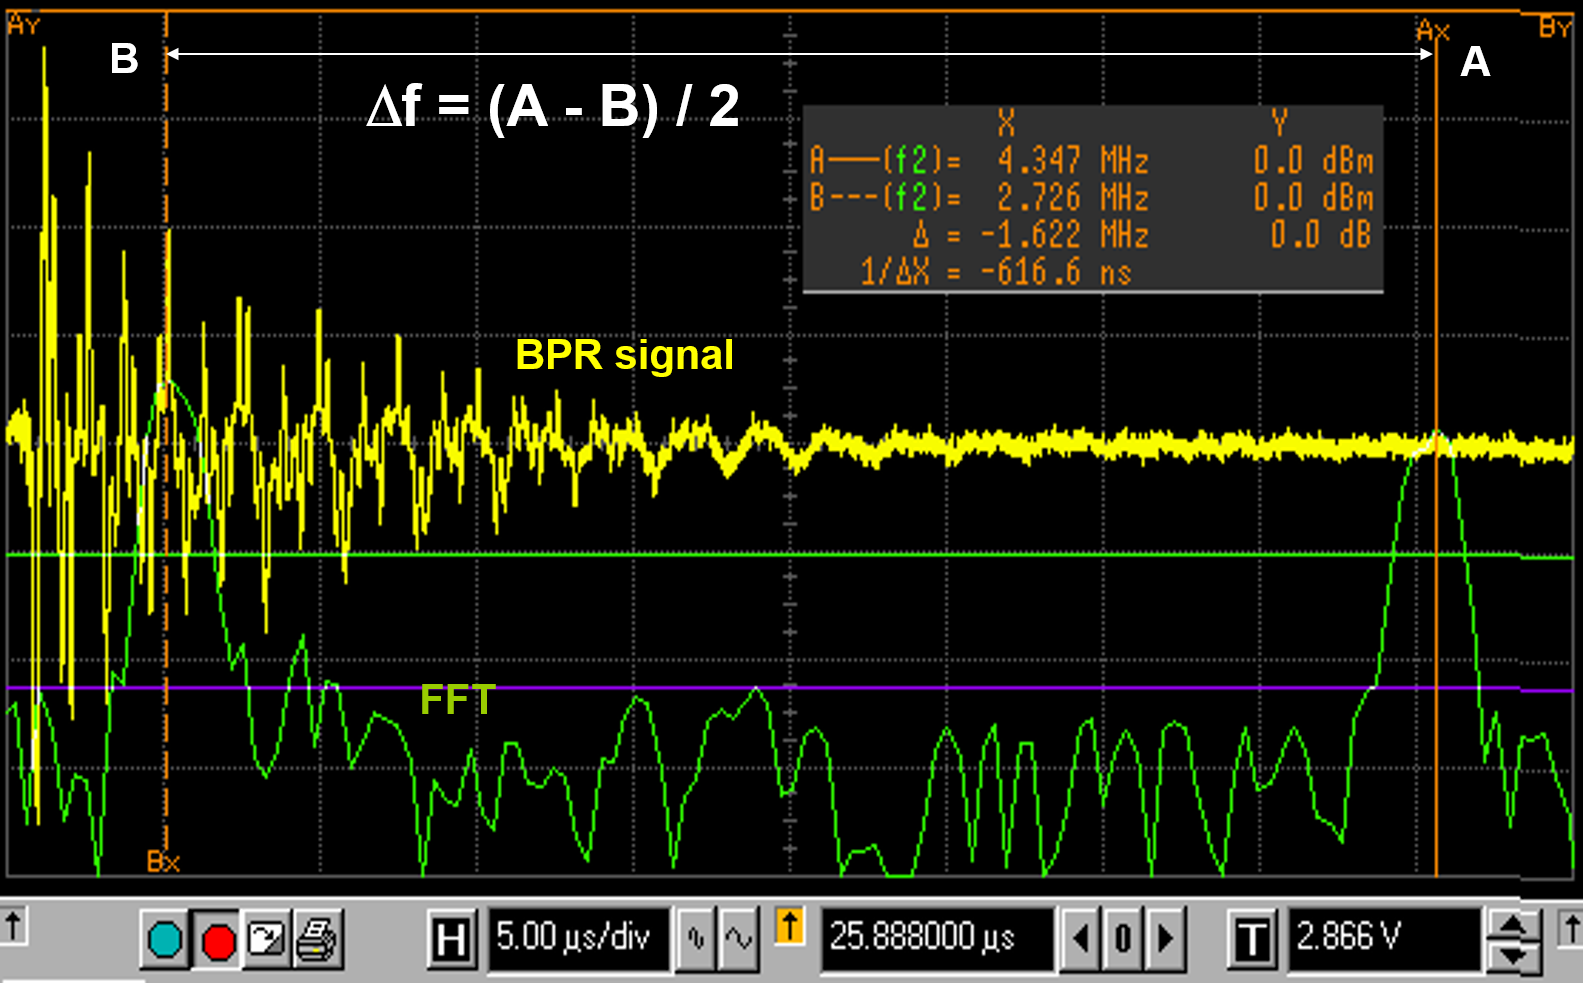
\includegraphics[width=0.55\columnwidth]{crlenbprspectrum.png}
  \label{fig:crlenbprspectrum}
  }
\subfloat[]
 {
  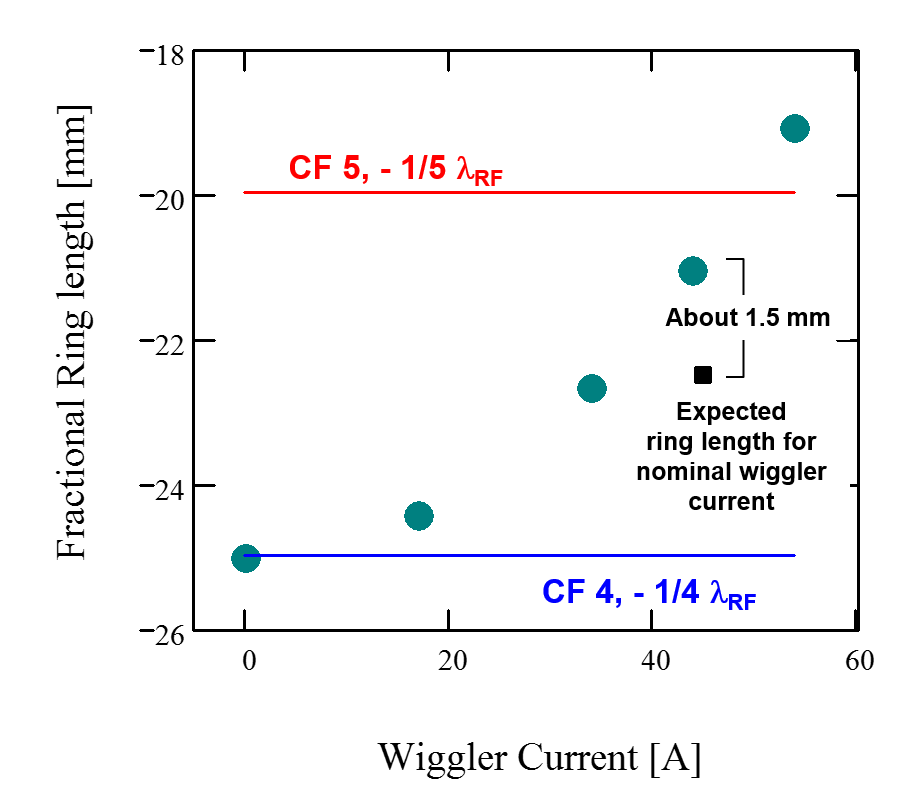
\includegraphics[width=0.4\columnwidth]{crlen.png}
  \label{fig:crlen}
 }
\caption[]{ BPR trace and its spectrum for circa 200~ns beam pulse circulating in the CR.
            Measured $L_{frac}=1/CF \lambda_{RF}$}
 
\end{figure}

In the Delay Loop this technique could not be used and the direct BPR measurements were employed.
The phase of reference signal was adjusted such that that the measured phase of the incoming beam
was zero and the wiggler setting was tuned that it was the same for the beam passing through the DL.

